\chapter{Testování}\label{ch:testing}

\chaptersummary{
   \begin{ul}
      \item krátké zdůvodnění vybraných typů testování \g{IS},
      \item popis automatizace testování v projektu.
   \end{ul}
}

Vzhledem k méně komplexní struktuře \g{IS} – malý počet mikroslužeb s poskytováním pouze \g{REST} rozhraní a jednoduchý základ klientské aplikace – příliš detailní testovací metody nejsou vhodné, zvětšovaly by časové náklady, ale nepřinášely žádnou výhodu.
Veškeré testování se proto omezilo na následující způsoby:

\begin{dl}
   \item[Statická analýza kódu] – s pomocí nástrojů \h{eslint} a \h{prettier} byla zajištěna konzistence vzhledu a metodika psaní implementovaných částí.
   Kontrola se týká především \h{.ts} a \h{.js} souborů.
   \item[Jednotkové testování] – ačkoliv takových testů není hodně, vzhledem k malému počtu samostatných funkcionalit vyčleněných do funkcí, pro každou mikroslužbou je nastaven \h{Jest} framework s možností kontroly pokrytí kódu testy.
   \item[Funkční testování] – pro funkční testování jsou poskytovány automaticky vytvářené testovací účty uživatelů s různými rolemi.
   Testy jsou realizovány ve formě jednotlivých testovacích scénářů s pomocí \h{Jest} frameworku.
   Taková forma testů má za úkol testovat přístupová práva jednotlivých přístupových bodů, validace dat a sekvence volání \g{REST} rozhraní nad celým systémem.
\end{dl}

\newpage

Za potenciálně vhodné, ale nevyužité, jsou považovány následující testovací metody:

\begin{dl}
   \item[Intergrační testy \g{MS}] – kontrola integrací konkrétní mikroslužby by byla vhodná při větším počtu mikroslužeb, kdy spuštění celého systému by bylo příliš nákladné.
   V takovém případě by bylo třeba vytvořit mock-funkcionalitu všech prvků, se kterou testovaná \g{MS} pracuje, a spustit je v samostatném prostředí.
   Toto testování je v aktuálním řešení nahrazeno funkčními testy celého \g{IS}, které plní stejný účel.
   \item[Zátěžové testy] – kontrola zátěže by byla přínosná pro odladění systému, avšak vyžaduje víc lokálních, případně vzdálených, prostředků pro testování.
   Nebylo zavedeno vzhledem k předpokládaným nevypovídajícím výsledkům s ohledem na~používané prostředí.
   \item[Testování klientského rozhraní] – vizuální rozhraní bylo dle specifikace psáno s omezeními (pouze jeden prohlížeč a pouze vysoké rozlišení obrazovky), plnohodnotné testování webového prostředí by zde nebylo v aktuální situaci vhodné.
   Takové testování bude potřeba v případě dokončení responzivního webového rozhraní, například s pomocí \h{cypress} balíčku.
\end{dl}



\section{Automatizace}\label{sec:automatization}

Na základě vybraných testů mohly být plně zautomatizovány pouze statická analýza kódu a jednotkové testy.
Kontrola kvality je integrována s pomocí \h{git hooks} a spouští se během každé tvorby \h{commit} prvku.
Jednotkové testy jsou řešeny obdobně, ale spouštění je prováděno až při každé \h{git push} akci na server.

Funkční testování je v dáno v podobě samostatného repozitáře a vzhledem k vazbě na celý systém a potřebě fungování všech částí, je lepší to z úplné automatizace vynechat.
Implementované testy pokryvaji dokončenou funkcionalitu systému, část výsledku automatizovaného testování je vidět na obrázku~\ref{fig:int-test}.


\begin{figure}[htbp]
   \centering
   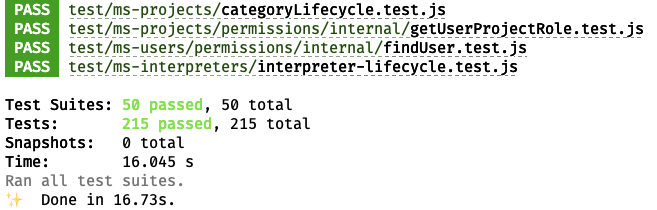
\includegraphics[max width=\textwidth]{assets/testing}
   \caption{Výsledek funkčních testů API}\label{fig:int-test}
\end{figure}
